% Options for packages loaded elsewhere
\PassOptionsToPackage{unicode}{hyperref}
\PassOptionsToPackage{hyphens}{url}
\PassOptionsToPackage{dvipsnames,svgnames,x11names}{xcolor}
%
\documentclass[
  letterpaper,
  DIV=11,
  numbers=noendperiod]{scrreport}

\usepackage{amsmath,amssymb}
\usepackage{iftex}
\ifPDFTeX
  \usepackage[T1]{fontenc}
  \usepackage[utf8]{inputenc}
  \usepackage{textcomp} % provide euro and other symbols
\else % if luatex or xetex
  \usepackage{unicode-math}
  \defaultfontfeatures{Scale=MatchLowercase}
  \defaultfontfeatures[\rmfamily]{Ligatures=TeX,Scale=1}
\fi
\usepackage{lmodern}
\ifPDFTeX\else  
    % xetex/luatex font selection
\fi
% Use upquote if available, for straight quotes in verbatim environments
\IfFileExists{upquote.sty}{\usepackage{upquote}}{}
\IfFileExists{microtype.sty}{% use microtype if available
  \usepackage[]{microtype}
  \UseMicrotypeSet[protrusion]{basicmath} % disable protrusion for tt fonts
}{}
\makeatletter
\@ifundefined{KOMAClassName}{% if non-KOMA class
  \IfFileExists{parskip.sty}{%
    \usepackage{parskip}
  }{% else
    \setlength{\parindent}{0pt}
    \setlength{\parskip}{6pt plus 2pt minus 1pt}}
}{% if KOMA class
  \KOMAoptions{parskip=half}}
\makeatother
\usepackage{xcolor}
\setlength{\emergencystretch}{3em} % prevent overfull lines
\setcounter{secnumdepth}{-\maxdimen} % remove section numbering
% Make \paragraph and \subparagraph free-standing
\ifx\paragraph\undefined\else
  \let\oldparagraph\paragraph
  \renewcommand{\paragraph}[1]{\oldparagraph{#1}\mbox{}}
\fi
\ifx\subparagraph\undefined\else
  \let\oldsubparagraph\subparagraph
  \renewcommand{\subparagraph}[1]{\oldsubparagraph{#1}\mbox{}}
\fi


\providecommand{\tightlist}{%
  \setlength{\itemsep}{0pt}\setlength{\parskip}{0pt}}\usepackage{longtable,booktabs,array}
\usepackage{calc} % for calculating minipage widths
% Correct order of tables after \paragraph or \subparagraph
\usepackage{etoolbox}
\makeatletter
\patchcmd\longtable{\par}{\if@noskipsec\mbox{}\fi\par}{}{}
\makeatother
% Allow footnotes in longtable head/foot
\IfFileExists{footnotehyper.sty}{\usepackage{footnotehyper}}{\usepackage{footnote}}
\makesavenoteenv{longtable}
\usepackage{graphicx}
\makeatletter
\def\maxwidth{\ifdim\Gin@nat@width>\linewidth\linewidth\else\Gin@nat@width\fi}
\def\maxheight{\ifdim\Gin@nat@height>\textheight\textheight\else\Gin@nat@height\fi}
\makeatother
% Scale images if necessary, so that they will not overflow the page
% margins by default, and it is still possible to overwrite the defaults
% using explicit options in \includegraphics[width, height, ...]{}
\setkeys{Gin}{width=\maxwidth,height=\maxheight,keepaspectratio}
% Set default figure placement to htbp
\makeatletter
\def\fps@figure{htbp}
\makeatother

\KOMAoption{captions}{tableheading}
\makeatletter
\makeatother
\makeatletter
\@ifpackageloaded{bookmark}{}{\usepackage{bookmark}}
\makeatother
\makeatletter
\@ifpackageloaded{caption}{}{\usepackage{caption}}
\AtBeginDocument{%
\ifdefined\contentsname
  \renewcommand*\contentsname{Table of contents}
\else
  \newcommand\contentsname{Table of contents}
\fi
\ifdefined\listfigurename
  \renewcommand*\listfigurename{List of Figures}
\else
  \newcommand\listfigurename{List of Figures}
\fi
\ifdefined\listtablename
  \renewcommand*\listtablename{List of Tables}
\else
  \newcommand\listtablename{List of Tables}
\fi
\ifdefined\figurename
  \renewcommand*\figurename{Figure}
\else
  \newcommand\figurename{Figure}
\fi
\ifdefined\tablename
  \renewcommand*\tablename{Table}
\else
  \newcommand\tablename{Table}
\fi
}
\@ifpackageloaded{float}{}{\usepackage{float}}
\floatstyle{ruled}
\@ifundefined{c@chapter}{\newfloat{codelisting}{h}{lop}}{\newfloat{codelisting}{h}{lop}[chapter]}
\floatname{codelisting}{Listing}
\newcommand*\listoflistings{\listof{codelisting}{List of Listings}}
\makeatother
\makeatletter
\@ifpackageloaded{caption}{}{\usepackage{caption}}
\@ifpackageloaded{subcaption}{}{\usepackage{subcaption}}
\makeatother
\makeatletter
\@ifpackageloaded{tcolorbox}{}{\usepackage[skins,breakable]{tcolorbox}}
\makeatother
\makeatletter
\@ifundefined{shadecolor}{\definecolor{shadecolor}{rgb}{.97, .97, .97}}
\makeatother
\makeatletter
\makeatother
\makeatletter
\makeatother
\ifLuaTeX
  \usepackage{selnolig}  % disable illegal ligatures
\fi
\IfFileExists{bookmark.sty}{\usepackage{bookmark}}{\usepackage{hyperref}}
\IfFileExists{xurl.sty}{\usepackage{xurl}}{} % add URL line breaks if available
\urlstyle{same} % disable monospaced font for URLs
\hypersetup{
  pdfauthor={Malvika Sharan},
  colorlinks=true,
  linkcolor={blue},
  filecolor={Maroon},
  citecolor={Blue},
  urlcolor={Blue},
  pdfcreator={LaTeX via pandoc}}

\author{Malvika Sharan}
\date{2021-10-12}

\begin{document}
\ifdefined\Shaded\renewenvironment{Shaded}{\begin{tcolorbox}[frame hidden, borderline west={3pt}{0pt}{shadecolor}, sharp corners, interior hidden, boxrule=0pt, enhanced, breakable]}{\end{tcolorbox}}\fi

\renewcommand*\contentsname{Table of contents}
{
\hypersetup{linkcolor=}
\setcounter{tocdepth}{2}
\tableofcontents
}
\bookmarksetup{startatroot}

\hypertarget{foundational-community-building}{%
\chapter{Foundational Community
Building}\label{foundational-community-building}}

\textbf{DRAFT PRE-ALPHA VERSION FOR ONLINE WEBPAGE}

\begin{quote}
\emph{We cannot expect to engage with and refer to communities unless we
first support them to be built from the inside out. `Community' should
be understood as a verb, not a noun, in other words, it is the
consequence of our efforts.} - Cormac Russell, Rikindling Democracy
\end{quote}

\hypertarget{building-communities-with-a-sense-of-purpose-and-belonging}{%
\section{Building communities with a sense of purpose and
belonging}\label{building-communities-with-a-sense-of-purpose-and-belonging}}

Community building is a process of enabling members in our communities
to move from the position of spectators or users to developers and
leaders in the project. Community managers or members in community
coordination roles identify and build meaningful pathways for everyone
to gain access to the skills and resources they need to participate in
the community. They carry out project-specific technical roles alongside
emergent and often non-quantifiable and invisible responsibilities in
the community needed to make the quality and visible work of their
communities effective. These background works involve approaches for
collaboration, maintenance, acknowledgement and capturing the impact of
community members' work - skills that can be learned and systematically
applied to all research work.

This training material has been designed to discuss foundational skills
through four modules, each designed for short-form project-based
discussion:

\begin{itemize}
\tightlist
\item
  \textbf{Module 1: 🚧} Community foundation: What is your community's
  story, who started it, what was the reason/purpose and where do we
  want to take it?
\item
  \textbf{Module 2: 🔤} Community of Practice basics: Purpose and
  outcomes, stakeholder mapping, roles and responsibility documentation
  and communication channels
\item
  \textbf{Module 3: 🗺} Community engagement: information mapping, a
  mountain of engagement, incentives and value-exchange
\item
  \textbf{Module 4: 📜} Creating and communicating your community
  charter: vision, mission, milestones, roadmap, ways of working
\end{itemize}

\hypertarget{contact}{%
\section{Contact}\label{contact}}

For any organisation-related queries or concerns, you can directly reach
out to me, Malvika Sharan, by emailing
\href{mailto:msharan@turing.ac.uk}{\nolinkurl{msharan@turing.ac.uk}}.
You can find more about me via my
\href{https://malvikasharan.github.io/}{homepage}, and follow me on
\href{https://twitter.com/MalvikaSharan}{Twitter} for rare moments where
I share something (which has reduced significantly in 2023!)

\hypertarget{license-and-credits}{%
\section{License and credits}\label{license-and-credits}}

This work is licensed under the MIT license (code) and Creative Commons
Attribution 4.0 International license (for documentation). You are free
to share and adapt the material for any purpose, even commercially, as
long as you provide attribution (give appropriate credit, provide a link
to the license, and indicate if changes were made) in any reasonable
manner, but not in any way that suggests the licensor endorses you or
your use, and with no additional restrictions.

\emph{All referenced resources when reused should be attributed
correctly.}

\bookmarksetup{startatroot}

\hypertarget{session-1-community-narrative}{%
\chapter{Session 1: 🚧 Community
Narrative}\label{session-1-community-narrative}}

\textbf{DRAFT PRE-ALPHA VERSION FOR ONLINE WEBPAGE}

\begin{quote}
\emph{I've learned that people will forget what you said, people will
forget what you did, but people will never forget how you made them
feel.} - Maya Angelou
\end{quote}

\hypertarget{key-lessons}{%
\section{Key lessons}\label{key-lessons}}

\begin{itemize}
\tightlist
\item
  Understanding your community's narrative
\item
  Identifying the main stakeholders who hold historical knowledge about
  the community
\item
  Documenting the reason/purpose of the initial vision and where the
  current stakeholders want to take the community
\end{itemize}

\hypertarget{part-1-community-and-community-of-practice-cop}{%
\section{🖥 Part 1: Community and Community of Practice
(CoP)}\label{part-1-community-and-community-of-practice-cop}}

\href{https://docs.google.com/presentation/d/1FlBt454su5wmELNfua_1EpoStjgzm4G7emKki-cuTBg/edit?usp=sharing}{\textbf{{[}Link
to the Google Slides{]}}}

\textbf{Example 1}

\_ \textbf{In 2012 at an office party, two employees exchanged their
interest in} \_ \emph{growing vegetables and flowers. They decided to
set up an interest group who would like to exchange their tips, tricks
and produce from their gardens/farms. Within a few months, they set up
an Instagram to post pictures of their products to share online. Next
year, more members joined them by renting an allotment near their office
space and met after work to go to the allotment and grow vegetables
together. Following summer, a few members wrote a proposal for their
organisation to fund their group to pay for the allotment rent, purchase
common tools and seeds and support their group to improve socialisation.
Now, every year their organisation hosts a yearly harvest party where
produce from the shared allotment is sold to the staff members to raise
funds for a local charity. Their music band plays live music and a
baking group shares free cakes and tea to engage more people at this
event.}

\textbf{Example 2}

\_ \textbf{In 2019, two employees exchanged their scientific goals for}
\_ \emph{open science training for people in the biology field. They
connected with another member who had a similar interest to write a
proposal to join an accelerator programme and build a project that will
allow them to train and mentor early career researchers in open science.
Soon, they launched their programme and opened a call for experts in
their area to join as mentors. In 2020, they received 20 applications
from researchers interested in receiving training. The program's success
attracted 60 applications the next year and the previous trainees joined
to mentor the next group. In 2021, they received grants to hire people,
provide funding to their participants and scale their effort by offering
this programme to people in other research fields. Now their trainees
are not only mentors but also trainers of this programme in their
network and frequently answer questions from new members.}

\textbf{Example 3}

\_ \textbf{In 2018 at a Data Study Group workshop, two industry leaders,
one from academia and one from the private sector, exchanged their
interest in each other's work} \_ \emph{in AI and Health Research. They
went back to their organisations to find organisation buy-in to set a
formal collaboration so that researchers across these organisations can
collaborate on exciting and innovative ideas that advance each
organisation's mission and reputation as industry leaders. They invested
funding to hire community managers and researchers to work in the
interface of their organisation. Soon, they launched engagement
initiatives and opened a call for experts in their area to apply for
funding schemes on topics of shared interest. They were successful in
their first year, and are excited about the possibility of the next 5
years.}

\hypertarget{open-discussions}{%
\subsection{Open discussions}\label{open-discussions}}

\begin{itemize}
\tightlist
\item
  \textbf{What trend do we see in these two scenarios?}
\item
  \textbf{What are the differences?}
\end{itemize}

\hypertarget{starting-with-why}{%
\subsection{Starting with ``Why''?}\label{starting-with-why}}

\begin{itemize}
\tightlist
\item
  Why does the project need a community?
\item
  Why did you take on this community role?
\item
  Why would others join this community?
\item
  How do these different sets of `purpose' align?
\end{itemize}

\hypertarget{silent-note-taking-using-prompts}{%
\subsubsection{\texorpdfstring{\textbf{Silent note-taking using
prompts}}{Silent note-taking using prompts}}\label{silent-note-taking-using-prompts}}

\textbf{1. Why does the project need a community?}

\begin{itemize}
\tightlist
\item
  What is your community project's story, who started it? Why is it
  important to build this community? - \textbf{What is the purpose?}
\item
  Reflecting on the status of your project, where next do you want to
  take your community/project? \textbf{What is the next step}, and what
  resources do you need to make that happen?
\end{itemize}

\textbf{2. Why do you or those who started the project care about
community and community/your role? Why would others join this
community?}

\begin{itemize}
\tightlist
\item
  There will be a combination of multiple reasons why you or those
  leading the project chose to support the community and community
  management. Let's start by sharing the reasons (from what you know
  about the project) that are most important to you.
\item
  What is one of the most rewarding community experiences you have had?
  (one that made you feel included or valued for your
  contribution/participation!) -- Reflecting on your experiences, why do
  you think people will join your community? What experience do you want
  them to have?
\end{itemize}

\hypertarget{aligning-your-communitys-purpose-with-the-organisations-motivation-for-community-management}{%
\subsection{Aligning your community's `purpose' with the organisation's
motivation for community
management}\label{aligning-your-communitys-purpose-with-the-organisations-motivation-for-community-management}}

\begin{figure}

{\centering 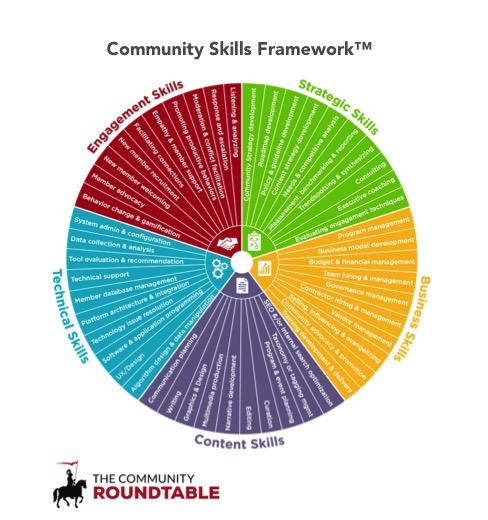
\includegraphics{quarto_files/images/CommunitySkillsFramework-TheCR.jpg}

}

\caption{Community Skills Framework - shown as a wheel with five main
areas of skills that a community manager may use - Engagement Skills,
technical skills, content skills, business skills amd strategic skills}

\end{figure}

\textbf{Reference:}
\url{https://communityroundtable.com/what-we-do/models-and-frameworks/community-skills-framework/}

\begin{itemize}
\tightlist
\item
  What skills and resources does your community have
\item
  What skills and resources do the project team including you have
\item
  What gaps exist - skills and resources do you and your team or
  community need
\item
  What up-skilling for your community, you and your team will be needed
\item
  Who from outside your community should be invited to fill those gaps
\end{itemize}

\textbf{Knowing what you know through your responses to these prompts,
what goals in your projects will you prioritise?}

\hypertarget{assignment}{%
\section{\texorpdfstring{📝
\textbf{Assignment:}}{📝 Assignment:}}\label{assignment}}

\href{https://docs.google.com/document/d/1BjicBMiOIwcG_L-foD1XPVV3b3s6-lKt8DtGoOAKvjg/edit?usp=sharing}{1
- Community background}\textbf{← {[}MAKE A COPY{]}}

\emph{Identify the origin story of the community that existed before you
joined. Interview key stakeholders in your project to fill any gaps your
narrative may have. This process will help identify your community's
mission, purpose and possible pathways you want to build.}

📑 \textbf{Reading recommendation:}

\begin{itemize}
\tightlist
\item
  The Turing Way - Managing a new community:
  \url{https://the-turing-way.netlify.app/collaboration/new-community.html}
\item
  Community Roundtable - Community Skills Framework:
  \url{https://communityroundtable.com/what-we-do/models-and-frameworks/community-skills-framework/}
\end{itemize}

\hypertarget{key-takeaways}{%
\section{🏡 Key takeaways}\label{key-takeaways}}

We reflected on the following aspects:

\begin{itemize}
\tightlist
\item
  Why it is important to start with ``Why'', the original purpose of
  your community
\item
  Why did you or those who started the community care about community
  and community/your role
\item
  Why build a strong and authentic narrative for your community - the
  reason why would others join this community
\item
  How to align your community's `purpose' with the organisation's
  motivation for community management
\end{itemize}

\bookmarksetup{startatroot}

\hypertarget{session-2-community-of-practice-basics}{%
\chapter{Session 2: 🔤 Community of Practice
Basics}\label{session-2-community-of-practice-basics}}

\textbf{DRAFT PRE-ALPHA VERSION FOR ONLINE WEBPAGE}

\begin{quote}
\emph{As a community, great things can happen when each individual
contributes, according to their strengths, toward a common goal.} ―
Idowu Koyenikan
\end{quote}

\hypertarget{key-lessons-1}{%
\section{Key lessons}\label{key-lessons-1}}

\begin{itemize}
\tightlist
\item
  Purpose and outcomes of your community
\item
  Creating a stakeholder map
\item
  Developing roles and responsibility documentation
\item
  Community communication channels
\end{itemize}

\hypertarget{part-2.1-mapping-stakeholders-and-their-engagement-needs}{%
\section{🖥 Part 2.1: Mapping Stakeholders and their engagement
needs}\label{part-2.1-mapping-stakeholders-and-their-engagement-needs}}

\href{https://docs.google.com/presentation/d/18kxCLkNEZBVfZ-IBMkE_Un0W67MBoEPbGabygMvqeRY/edit\#slide=id.g13faa93073d_0_111}{\textbf{Link
to the Google Slides}}

\hypertarget{lets-first-start-by-reflecting-on-these-questions}{%
\subsection{Let's first start by reflecting on these
questions}\label{lets-first-start-by-reflecting-on-these-questions}}

\begin{itemize}
\tightlist
\item
  Why invest in community building?
\item
  What are some good examples of community building have you
  experienced?
\end{itemize}

\hypertarget{purpose-and-outcomes}{%
\subsection{\texorpdfstring{\textbf{Purpose and
outcomes}}{Purpose and outcomes}}\label{purpose-and-outcomes}}

\emph{Each participant can create a table to add details from their
projects.}

\begin{longtable}[]{@{}lll@{}}
\toprule\noalign{}
\textbf{Project/subproject Names} & \textbf{Purpose} &
\textbf{Outcomes} \\
\midrule\noalign{}
\endhead
\bottomrule\noalign{}
\endlastfoot
& & \\
& & \\
& & \\
\end{longtable}

\hypertarget{identifying-stakeholders}{%
\subsection{\texorpdfstring{\textbf{Identifying
Stakeholders}}{Identifying Stakeholders}}\label{identifying-stakeholders}}

\begin{longtable}[]{@{}lll@{}}
\toprule\noalign{}
\textbf{Contributors} & \textbf{Role} & \textbf{Nature of
participation} \\
\midrule\noalign{}
\endhead
\bottomrule\noalign{}
\endlastfoot
& & \\
& & \\
& & \\
\end{longtable}

\hypertarget{optional-for-projects-with-many-stakeholders-prioritising-stakeholders}{%
\subsection{\texorpdfstring{\textbf{2.2 Optional for projects with many
stakeholders: Prioritising
Stakeholders}}{2.2 Optional for projects with many stakeholders: Prioritising Stakeholders}}\label{optional-for-projects-with-many-stakeholders-prioritising-stakeholders}}

\href{https://docs.google.com/presentation/d/1BO-_VtRL-WrcpoEzSv_4ZCcEEg8QaZepeRGx6rB9grQ/edit\#slide=id.g1072083f421_1_0}{\textbf{Link
to the Google Slides}}

Anybody who can affect or is affected by an organisation, project,
community or the processes and strategy they use. Identifying who they,
how they engage and what they need to affect changes is crucial for the
success of a project.

\begin{figure}

{\centering 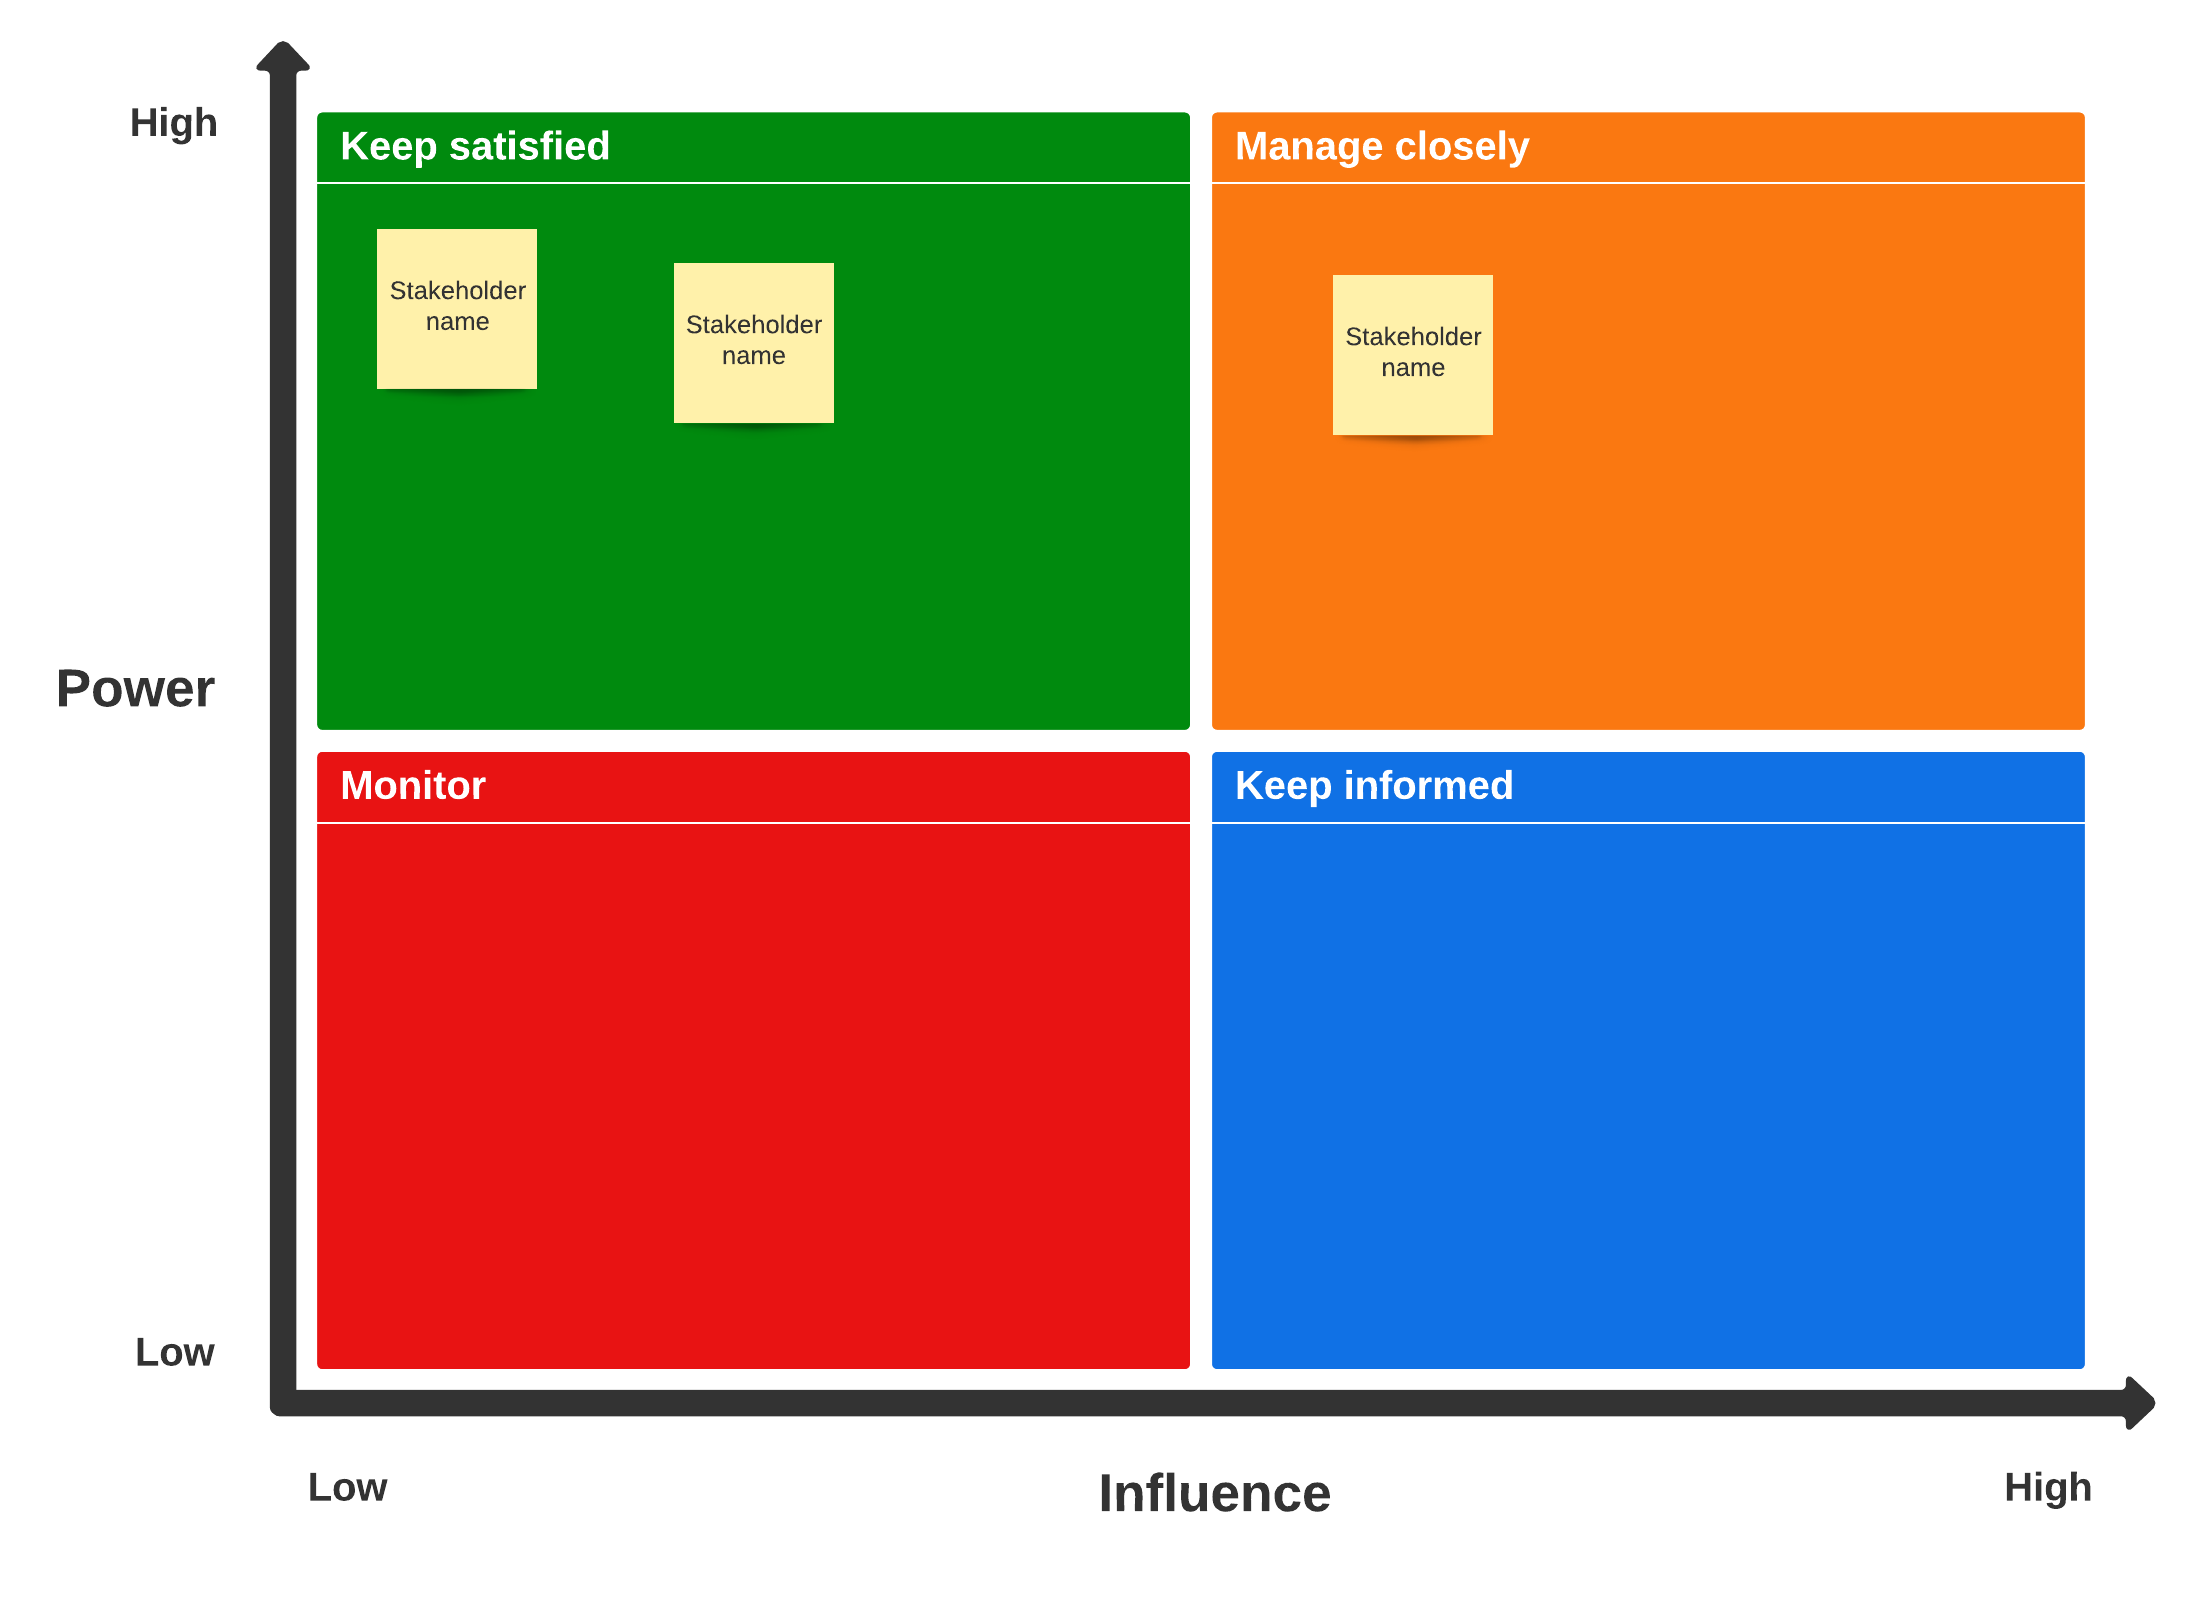
\includegraphics{quarto_files/images/stakeholder-map-lucidspark.png}

}

\caption{Stakeholder map example with four quadrants - Keep satisfied
(high power, low interest), Manage closely (high power, high interest),
Inform regularly (low power, high interest), Monitor and anticipate
needs (low power, low interest)}

\end{figure}

\textbf{Template for the Community Management at the Turing}

\href{https://miro.com/app/board/uXjVMWzhGGc=/?share_link_id=996948844923}{Extanded
Miro Board for Stakeholder and Communication/Engagement Mapping}

\textbf{Find general templates for reuse:}

\begin{itemize}
\tightlist
\item
  Lucidparks:
  \url{https://lucidspark.com/blog/a-guide-to-stakeholder-mapping}
\item
  Mural: \url{https://www.mural.co/templates/stakeholder-mapping}
\item
  Miro: \url{https://miro.com/templates/stakeholder-map/}
\end{itemize}

\hypertarget{resources-and-engagementcommunication-platforms}{%
\subsection{\texorpdfstring{\textbf{2.3 Resources and
engagement/communication
platforms}}{2.3 Resources and engagement/communication platforms}}\label{resources-and-engagementcommunication-platforms}}

\textbf{Resources and infrastructure:}

\begin{itemize}
\tightlist
\item
  Tools/platforms:
\item
  Documentation:
\item
  Infrastructure:
\item
  Events:
\item
  Opportunities:
\item
  Agency and decision-making power:
\item
  \protect\hyperlink{anything-else}{Anything else?}
\end{itemize}

\textbf{Types of engagement:}

\begin{itemize}
\tightlist
\item
  Primary: GitHub
\item
  Asynchronous: Newsletter, talks, Slack, Twitter, documentation
\item
  Synchronous: Co-working calls, Collaboration Cafe, Book Dash
\item
  \emph{Let's discuss the other types of engagements you have
  implemented \ldots{}}
\end{itemize}

\hypertarget{assignment-2-discussions}{%
\section{\texorpdfstring{📝 \textbf{Assignment 2 +
Discussions:}}{📝 Assignment 2 + Discussions:}}\label{assignment-2-discussions}}

\href{https://docs.google.com/document/d/1r08Yu2tG8DcOiMpF6bbHrlgMRdePNxlWSRd3tvK7fcQ/edit?usp=sharing}{2
- Community of Practice Basics} \textbf{← {[}MAKE A COPY{]}}

\begin{enumerate}
\def\labelenumi{\arabic{enumi}.}
\tightlist
\item
  What is the purpose of your CoP or project? What are the main and
  expected outcomes of the project?
\item
  Who are your stakeholders and what are their roles?
\item
  How do you facilitate their participation, collaboration and
  contributions - what are the engagement and communication platforms?
\end{enumerate}

\textbf{Reading recommendation}

\begin{itemize}
\tightlist
\item
  Research culture: let's reimagine how we work together:
  \url{https://wellcome.org/what-we-do/our-work/research-culture}
\end{itemize}

\textbf{Note:}

\begin{itemize}
\tightlist
\item
  The assignments from this session is for you to come back to, update
  and reflect on periodically, such as in the mid-year or annual review.
\item
  You can exchange this with other community managers to get some
  feedback.
\end{itemize}

\hypertarget{key-takeaways-1}{%
\section{🏡 Key takeaways}\label{key-takeaways-1}}

In this session, we discussed:

\begin{itemize}
\tightlist
\item
  How to map the purpose and outcome of your community
\item
  How to map stakeholders and their engagement in the project
\item
  how to enable that engagement through appropriate communications
  tools, channels and platforms
\end{itemize}

\bookmarksetup{startatroot}

\hypertarget{session-3-community-engagement}{%
\chapter{Session 3: 🗺 Community
Engagement}\label{session-3-community-engagement}}

\textbf{DRAFT PRE-ALPHA VERSION FOR ONLINE WEBPAGE}

\begin{quote}
\emph{Just because you can draw a detailed map, doesn't mean you are
accurately representing the territory!} - Yuval Noah Harari
\end{quote}

\hypertarget{key-lessons-2}{%
\section{Key lessons}\label{key-lessons-2}}

\begin{itemize}
\tightlist
\item
  Information mapping for your community
\item
  Building a mountain/matrix of engagement
\item
  Understanding and mapping incentives and value-exchange
\end{itemize}

\hypertarget{part-3-community-participation-and-value-exchange}{%
\section{🖥 Part 3: Community participation and
Value-exchange}\label{part-3-community-participation-and-value-exchange}}

{[}\href{https://docs.google.com/presentation/d/11LH1edg_0srL2ibTl2mVnsICIydtT0i2WC93TsjacsM/edit\#slide=id.g13faa93073d_0_1507}{Link
to the Google slides}{]}

\hypertarget{to-ensure-equitable-community-participation-its-important-to-map-the-following-information}{%
\subsection{To ensure equitable community participation, it's important
to map the following
information:}\label{to-ensure-equitable-community-participation-its-important-to-map-the-following-information}}

\begin{itemize}
\tightlist
\item
  what different resources and processes in our community exist
\item
  what do different kinds of community participation and engagement look
  like
\item
  what values do we create for our community members to participate in
  our community and engage with our work
\item
  what processes work that can be used to iterate and improve all forms
  of participation and build a fair value exchange (support and
  acknowledgement) system
\end{itemize}

\hypertarget{we-will-utilise-the-mountainmatrix-of-engagement-to-map-community-processes-and-value-exchange}{%
\subsection{We will utilise the mountain/matrix of engagement to map
community processes and value
exchange:}\label{we-will-utilise-the-mountainmatrix-of-engagement-to-map-community-processes-and-value-exchange}}

\begin{itemize}
\tightlist
\item
  Discover how people interact with your community, organisation, or
  project and its culture.
\item
  Discover how people identify and move between different types of
  interactions.
\item
  Develop pathways for people to move from first contact to sustained
  engagement to leadership
\item
  Embed value-exchange and fair recognition process in the project
\end{itemize}

\hypertarget{assignment-1}{%
\section{\texorpdfstring{📝
\textbf{Assignment:}}{📝 Assignment:}}\label{assignment-1}}

\href{https://docs.google.com/document/d/1JtsNwZUHtSfKQKeyR36e97tgN8BR-MQEMx2MHNtBsYI/edit\#}{3
- community participation and engagement} \textbf{← {[}Make a Copy{]}}

\textbf{TODO:} Bring one or multiple of these resources to share with
others

\begin{itemize}
\tightlist
\item
  Your favourite community document - from your or another project -
  these documents could be an annual report, a community health report
  (how is your community doing, what are the indicators)
\item
  A community policy from your work (contributing guidelines, code of
  conduct etc.)
\item
  Strategy or communication document.
\end{itemize}

\textbf{Reading recommendation}

\begin{itemize}
\tightlist
\item
  Personas and Pathways:
  \url{https://the-turing-way.netlify.app/project-design/persona.html}
\item
  Jones, C. M. (2022). How to Reward Your Community Members And Keep
  Them Engaged. CMX.
  \url{https://cmxhub.com/how-to-reward-your-community-members}
\item
  Creating Pathways:
  \href{https://medium.com/@abbycabs/creating-pathways-that-invest-in-new-maintainers-8ffb52e09681}{Creating
  Pathways That Invest in New Maintainers}
\item
  Map is not the territory:
  \url{https://conceptually.org/concepts/the-map-is-not-the-territory}
\end{itemize}

\hypertarget{key-takeaways-2}{%
\section{🏡 Key takeaways}\label{key-takeaways-2}}

In this session, we discussed:

\begin{itemize}
\tightlist
\item
  The Mountain/Matrix of engagement to understand what different levels
  of engagement look like and how we facilitate that.
\item
  How do we move from one level to another? When to recognise someone
  can move from one band to another?
\item
  Mountain of Engagement should be a living document, reflecting on what
  your community experiences are and where you should modify them.
\end{itemize}

\bookmarksetup{startatroot}

\hypertarget{session-4-creating-and-communicating-community-charter}{%
\chapter{Session 4: 📜 Creating and Communicating Community
Charter}\label{session-4-creating-and-communicating-community-charter}}

\textbf{DRAFT PRE-ALPHA VERSION FOR ONLINE WEBPAGE}

\begin{quote}
\emph{Values are the rules by which we live -- the filters through which
we evaluate possible actions, the base upon which we make decisions in
support of the achievement of our collective and individual vision and
purpose.} -- Michael Cavanagh
\end{quote}

\hypertarget{key-lessons-3}{%
\section{Key lessons}\label{key-lessons-3}}

\begin{itemize}
\tightlist
\item
  Framing your community vision
\item
  Communicating your community mission
\item
  Defining roadmaps and milestones
\item
  Establishing ways of working
\end{itemize}

\hypertarget{part-4-personal-and-organisation-values}{%
\section{🖥 Part 4: Personal and Organisation
``Values''}\label{part-4-personal-and-organisation-values}}

\href{https://docs.google.com/presentation/d/1JZt3HQMKg_6Eu3ctHH3PUv-9LgdTwFpyYhkrOwf5AUs/edit?usp=sharing}{{[}Link
to the Google slides{]}}

``\emph{A goal is not always meant to be reached, it often serves simply
as something to aim at.'' ― Bruce Lee}

\hypertarget{lets-start-with-silent-reflections-and-notetaking-based-the}{%
\section{Let's start with silent reflections and notetaking based
the}\label{lets-start-with-silent-reflections-and-notetaking-based-the}}

\begin{itemize}
\tightlist
\item
  Identify your core values (pick 3 for this session) based on this
  \href{https://thehappinessplanner.co.uk/pages/list-of-core-values}{list
  of personal core values})
\item
  Choose one and define how you see it, Offer examples of your chosen
  value in action - share with others
\end{itemize}

\textbf{Personal Reflections}

\begin{itemize}
\tightlist
\item
  How do your values align with the work you do?
\item
  How would you help a contributor align their values, vision and goal?
\item
  What will this discussion between you and them look like?
\end{itemize}

\hypertarget{vision-articulating-your-big-ideas-for-the-future}{%
\section{Vision: Articulating your big ideas (for the
future)}\label{vision-articulating-your-big-ideas-for-the-future}}

Writing something short and succinct can take more time than multiple
sentences - it can be iteratively improved with other stakeholders
periodically.

\textbf{Prompts for vision}

\begin{quote}
What you are doing - Why you are doing this - the impact or change your
project will bring - Who are users and contributors
\end{quote}

\hypertarget{mission-where-you-are-right-now-what-your-objectives-are-what-is-next.}{%
\section{Mission: Where you are right now, what your objectives are,
what is
next.}\label{mission-where-you-are-right-now-what-your-objectives-are-what-is-next.}}

\textbf{Prompts for Mission}

\begin{quote}
What the objectives are - What does your project offers and what makes
it unique - What the next steps are (Process for community engagement
and project development)
\end{quote}

\hypertarget{roadmap-an-overview-of-the-projects-goals-and-outcomes-presented-on-a-timeline.}{%
\section{Roadmap: an overview of the project's goals and outcomes
presented on a
timeline.}\label{roadmap-an-overview-of-the-projects-goals-and-outcomes-presented-on-a-timeline.}}

\begin{itemize}
\tightlist
\item
  Roadmap is supplemented with details such as scope, resources, ways of
  working, risks
\item
  Roadmap does not provide task-level details. (For task-level details,
  see project charter).
\item
  Information gathered so far can be put together in a project charter,
  or maintained through separate documents. You can consider adding more
  details. (Prompts in the assignment)
\end{itemize}

\hypertarget{reflection-for-the-future}{%
\subsection{Reflection for the future}\label{reflection-for-the-future}}

\emph{Let's discuss what is the definition of success for your
communities in 6 months/12 months/2 years looks like based on where you
are right now.}

\hypertarget{assignment-4-discussions}{%
\section{\texorpdfstring{📝 \textbf{Assignment 4 +
Discussions:}}{📝 Assignment 4 + Discussions:}}\label{assignment-4-discussions}}

\begin{itemize}
\tightlist
\item
  Identify your community's values and represent them in all processes
  (policies, guidelines, onboarding, decision-making, communication
  etc.) through intentional efforts for ensuring inclusion and diversity
  in your community.
\end{itemize}

\href{https://docs.google.com/document/d/1c5NDGUnVc-L5DPop3UvpgOw3XuZHrY5B1wQ9mBWWoXg/edit?usp=sharing}{4
- Community Vision, Mission, Roadmap, Charter}\textbf{← {[}Make a
Copy{]}}

\textbf{Reading recommendation:}

\begin{itemize}
\tightlist
\item
  \href{https://drive.google.com/file/d/1dzTWPNXwPCAMZJBiEBf0a4c_y9F3Bvk1/view?usp=sharing}{6-AuthenticPrinciplesCommEng.pdf}
  \emph{(reference:}
  \href{https://www.health.state.mn.us/communities/practice/resources/phqitoolbox/authenticprinciples.html}{\emph{Principles
  of Authentic Community Engagement}} \emph{- Minnesota Dept. of Health.
  (2014, September 28).)}
\end{itemize}

\hypertarget{key-takeaways-3}{%
\section{🏡 Key takeaways}\label{key-takeaways-3}}

In this session, we learned how to:

\begin{itemize}
\tightlist
\item
  build a community charter
\item
  ensure clarity in your work through transparent documentation
\end{itemize}

\bookmarksetup{startatroot}

\hypertarget{logistics-for-facilitators-and-attendees}{%
\chapter{Logistics for Facilitators and
Attendees}\label{logistics-for-facilitators-and-attendees}}

This workshop session brings new community managers or members in
community coordination roles together in a cohort format to introduce
foundational skills for community management while encouraging them to
share skills, experiences and ideas for collaboration with each other.

Here is a recommendation for participants to help with keeping this
workshop series as interactive as possible while ensuring that every one
the chance to contribute to the discussion:

\begin{itemize}
\tightlist
\item
  If you generally take less space, please use this workshop to take
  more space.
\item
  If you generally take space, try to give space to others.
\item
  We will have many quiet reflections during the training.
\item
  Silence can be awkward but that is not a sign that others who are
  often not the first ones to speak have nothing to add.
\end{itemize}

\hypertarget{participation-guidelines-for-the-workshops}{%
\section{Participation guidelines for the
workshops}\label{participation-guidelines-for-the-workshops}}

\begin{itemize}
\tightlist
\item
  The workshop facilitator will introduce topics through a short
  presentation, followed by either a quiet assignment (by yourself) or
  breakout room (group discussion), followed by full group reflection
  and sharing insights.
\item
  We will use a shared web-based clock to ensure keeping discussions on
  time using Cuckoo Clock \href{https://cuckoo.team}{cuckoo.team}
  \textless-- update for you
\item
  A shared document will be set up for each session with information
  guiding the format, space for documenting notes collaboratively, and
  sharing resources (links, thoughts, examples)

  \begin{itemize}
  \tightlist
  \item
    You can leave and come back to the workshop as it suits
  \end{itemize}
\item
  We encourage sharing feedback to make sure that this and future
  sessions are beneficial for all of us.

  \begin{itemize}
  \tightlist
  \item
    If you experience something that makes you uncomfortable (topic,
    conversation or format of any certain session), please let me
    (Malvika) know privately (msharan@turing.ac.uk) so that I can act
    immediately.
  \end{itemize}
\item
  Each call will be paired with an assignment to help you reflect on the
  practices in the context of your project. We will allocate 10 minutes
  in the following call to share insights from our assignments with
  others. Although I can not make it mandatory for you to complete this
  assignment, it will be more effective if you take some to complete
  them. If you feel comfortable, you can share the links to your
  assignment in the shared document.
\end{itemize}

\hypertarget{format}{%
\section{Format}\label{format}}

\begin{itemize}
\tightlist
\item
  Lessons and shared documents are designed using examples from
  \href{https://foundation.mozilla.org/en/initiatives/mozilla-open-leaders/}{Mozilla
  Open Leaders Programme}
\item
  Each lesson has been designed for 1 hour.
\item
  Additional 20-30 minutes of the workshop sessions should be reserved
  for open discussion and for sharing insights from our assignments with
  others.
\item
  Lessons are provided in a format that can be copied directly on a
  shared document for teaching purposes.
\item
  Each lesson has been paired with practical assignments to help
  learners reflect on the practices in the context of their projects.
\item
  Before each lesson, please provide details such as date, time and
  joining link for the session, and create a space for feedback (pluses
  and delta) and reflections (such as what was the main takeaway for
  participants personally, what was not clear) at the end of each
  session.
\end{itemize}

\hypertarget{joining-the-call}{%
\subsection{Joining the call}\label{joining-the-call}}

\begin{itemize}
\tightlist
\item
  Please inform participants if the presentation part of this call can
  be recorded for people who are unable to attend this session.
\item
  The discussion part should not be recorded to allow honest and open
  discussion.
\end{itemize}

\hypertarget{roll-call}{%
\subsection{Roll call}\label{roll-call}}

For each session, I recommend using roll call with icebreaker questions
prompting reflections related to the content. Below is a suggestion for
each session:

\begin{itemize}
\tightlist
\item
  Session 1 icebreaker question: \emph{What is one characteristic about
  a community you most admire? Have you been able to replicate that for
  your project? If yes, how? If not, why not?}
\item
  Session 2 icebreaker question: \emph{Reflections from learning about
  your community and building a narrative - what was most surprising?}
\item
  Session 3 icebreaker question: \emph{Reflect on what you as a
  community builder/facilitator/participant bring into your community
  space and what do you receive+give back?\textbf{ (kindness, empathy,
  professional expertise, resources, technical knowledge, mentorship
  etc.) / }Does this balance seem right?}
\item
  Session 4 icebreaker question: From the
  \href{https://thehappinessplanner.co.uk/pages/list-of-core-values}{LIST
  OF PERSONAL CORE VALUES}, select and share three values based on your
  current work (this may change in the future)
\end{itemize}

\hypertarget{concluding-the-session}{%
\subsection{Concluding the Session}\label{concluding-the-session}}

At the end of the shared document for each session - you can ask for two
post-session inputs:

\begin{itemize}
\tightlist
\item
  Questions and suggestions (responses can be shared asynchronously
  through notes)
\item
  Feedback from the sessions: \_What worked? What didn't work? What
  would you change? What surprised you?
\end{itemize}

\hypertarget{below-are-some-potential-topics-for-additional-modules}{%
\section{Below are some potential topics for additional
modules:}\label{below-are-some-potential-topics-for-additional-modules}}

\begin{itemize}
\tightlist
\item
  \textbf{Open Science/research implementation}: applying open,
  equitable and participatory approaches for building communities
\item
  \textbf{Facilitating community events}: Good practices for online vs
  in person facilitation of community events
\item
  \textbf{Impact assessment and reporting}: What are some good practices
  and frameworks for impact assessment in the community, and how do we
  report them
\item
  \textbf{Conflict management} and handling a difficult situation

  \begin{itemize}
  \tightlist
  \item
    Positive Deviance. (2018, July 12):
    \url{https://involve.org.uk/resources/methods/positive-deviance}
  \item
    Code of Conduct and Restorative practice:
    \url{https://github.com/alan-turing-institute/open-community-building/blob/main/CODE_OF_CONDUCT.md\#6-restorative-practice-statement-and-principles}
  \item
    What is Conflict Management? \textbar{} peopleHum:
    \url{https://www.peoplehum.com/glossary/conflict-management}
  \item
    Restorative Practices -- Conflict Resolution Education Connection:
    \url{https://creducation.net/conflict_resolution_education_practice_areas/restorative_practices}
  \item
    The Positive Value of Conflict: The Power of Resolution:
    \url{https://www.psychologytoday.com/gb/blog/inside-out-outside-in/202103/the-positive-value-conflict-the-power-resolution}
  \end{itemize}
\end{itemize}

\hypertarget{anything-else}{%
\subsection{Anything else?}\label{anything-else}}

Have suggestions for more topics? Share them with me by emailing
\href{mailto:msharan@turing.ac.uk}{\nolinkurl{msharan@turing.ac.uk}}.

\textbf{\emph{Happy community building!}}



\end{document}
